% Attachment method cross-sections: cupillar_opt1 and sbump_sac305.
% The two stacks are separate, mutually exclusive methods. The solder ball is
% not an optional cap on a Cu pillar: it is its own method, with its own
% passivation opening, its own datatype and its own ADK adapter.
\documentclass[border=3mm]{standalone}
\usepackage{tikz}
\usetikzlibrary{arrows.meta, positioning, calc, decorations.pathreplacing}
\usepackage[T1]{fontenc}
\usepackage{lmodern}

% IHP Colors
\definecolor{IHPfg}{RGB}{0,80,139}
\definecolor{IHPaccent}{RGB}{109,112,114}
\definecolor{IHPlight}{RGB}{225,238,250}
\definecolor{cTM2}{RGB}{200,60,60}
\definecolor{cPass}{RGB}{160,160,165}
\definecolor{cCuPillar}{RGB}{184,115,51}
\definecolor{cSnAg}{RGB}{170,175,180}
\definecolor{cSolder}{RGB}{130,130,135}

\begin{document}
% Coordinates are in micrometres. The unit vectors compress the drawing to a
% readable size while keeping the two stacks on one common scale.
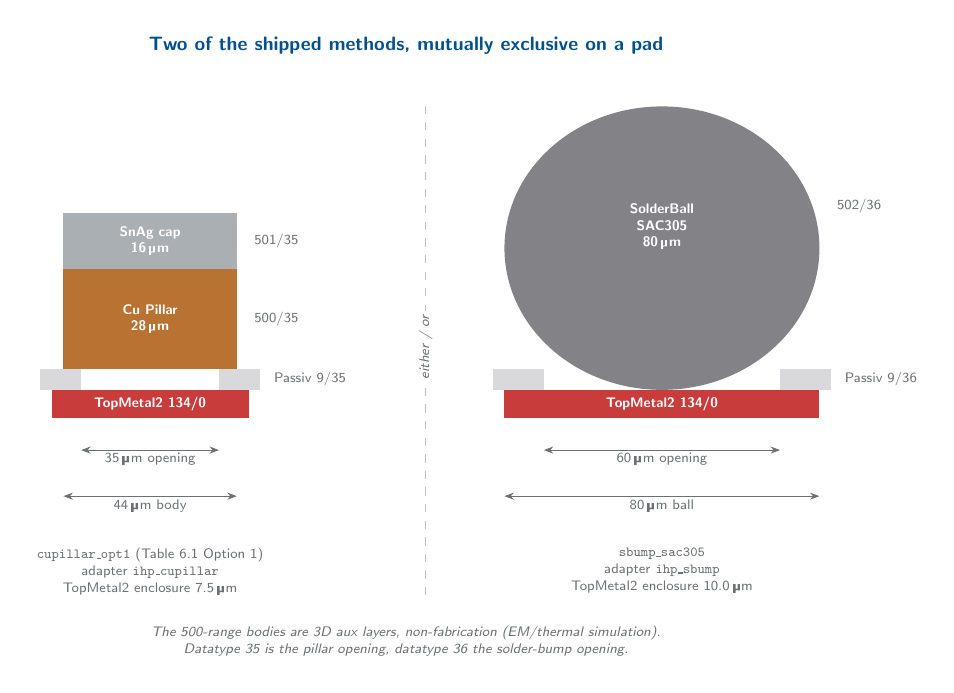
\begin{tikzpicture}[
    x=0.05cm, y=0.045cm,
    dim/.style={
        {Stealth[length=1.2mm]}-{Stealth[length=1.2mm]},
        line width=0.4pt, color=IHPaccent
    },
    dimlbl/.style={
        font=\sffamily\tiny, text=IHPaccent, fill=white, inner sep=1pt
    },
    layerlbl/.style={
        font=\sffamily\tiny\bfseries, text=white, align=center
    },
    gdslbl/.style={
        font=\sffamily\tiny, text=IHPaccent, anchor=west
    },
    caption/.style={
        font=\sffamily\tiny, text=IHPaccent, align=center, anchor=north
    }
]

% ======================================================================
% Left stack: cupillar_opt1 (Table 6.1 Option 1)
%   TopMetal2 pad 50 um (35 um opening + 2 x 7.5 um enclosure)
%   Cu pillar 28 um x 44 um, SnAg cap 16 um x 44 um
% ======================================================================

% TopMetal2 pad
\fill[cTM2] (-25, 0) rectangle (25, 8);
\node[layerlbl] at (0, 4) {TopMetal2 134/0};

% Cu pillar body
\fill[cCuPillar] (-22, 14) rectangle (22, 42);
\node[layerlbl] at (0, 28) {Cu Pillar\\28\,\textmu m};
\node[gdslbl] at (24, 28) {500/35};

% SnAg cap body
\fill[cSnAg] (-22, 42) rectangle (22, 58);
\node[layerlbl] at (0, 50) {SnAg cap\\16\,\textmu m};
\node[gdslbl] at (24, 50) {501/35};

% Passivation, drawn last so it occludes the body edges
\fill[cPass!40] (-28, 8) rectangle (-17.5, 14);
\fill[cPass!40] (17.5, 8) rectangle (28, 14);
\node[gdslbl] at (29, 11) {Passiv 9/35};

% Opening and body dimensions
\draw[dim] (-17.5, -9) -- (17.5, -9);
\node[dimlbl, below] at (0, -9) {35\,\textmu m opening};
\draw[dim] (-22, -22) -- (22, -22);
\node[dimlbl, below] at (0, -22) {44\,\textmu m body};

\node[caption] at (0, -34)
    {\textbf{\texttt{cupillar\_opt1}} (Table 6.1 Option 1)\\
     adapter \texttt{ihp\_cupillar}\\
     TopMetal2 enclosure 7.5\,\textmu m};

% ======================================================================
% Separator: the two methods are alternatives, never a single stack
% ======================================================================
\draw[IHPaccent!45, dashed, line width=0.4pt] (70, -50) -- (70, 88);
\node[font=\sffamily\tiny\itshape, text=IHPaccent, rotate=90,
      fill=white, inner sep=1.5pt] at (70, 20) {either / or};

% ======================================================================
% Right stack: sbump_sac305
%   TopMetal2 pad 80 um (60 um opening + 2 x 10 um enclosure)
%   SAC305 ball 80 um x 80 um, landing in the /36 opening
% ======================================================================

% TopMetal2 pad
\fill[cTM2] (90, 0) rectangle (170, 8);
\node[layerlbl] at (130, 4) {TopMetal2 134/0};

% SAC305 ball body
\fill[cSolder] (130, 48) ellipse (40 and 40);
\node[layerlbl] at (130, 54) {SolderBall\\SAC305\\80\,\textmu m};
\node[gdslbl] at (172, 60) {502/36};

% Passivation, drawn last so it occludes the ball edges
\fill[cPass!40] (87, 8) rectangle (100, 14);
\fill[cPass!40] (160, 8) rectangle (173, 14);
\node[gdslbl] at (174, 11) {Passiv 9/36};

% Opening and ball dimensions
\draw[dim] (100, -9) -- (160, -9);
\node[dimlbl, below] at (130, -9) {60\,\textmu m opening};
\draw[dim] (90, -22) -- (170, -22);
\node[dimlbl, below] at (130, -22) {80\,\textmu m ball};

\node[caption] at (130, -34)
    {\textbf{\texttt{sbump\_sac305}}\\
     adapter \texttt{ihp\_sbump}\\
     TopMetal2 enclosure 10.0\,\textmu m};

% ======================================================================
% Title and legend
% ======================================================================
\node[font=\sffamily\scriptsize\bfseries, text=IHPfg, anchor=south]
    at (65, 100) {Two of the shipped methods, mutually exclusive on a pad};

\node[font=\sffamily\tiny\itshape, text=IHPaccent, anchor=north, align=center]
    at (65, -56)
    {The 500-range bodies are 3D aux layers, non-fabrication
     (EM/thermal simulation).\\
     Datatype 35 is the pillar opening, datatype 36 the solder-bump opening.};

\end{tikzpicture}
\end{document}
